\documentclass{beamer}
\RequirePackage{luatex85}
\include{../style/cours-style.sty}

% Title
\title{Introduction au Développement Web - Bachelor CSI}
\author{Christophe Brun}
\institute{Campus Saint-Michel IT}
\date{25 juin 2024}
\beamertemplatenavigationsymbolsempty

\titlegraphic{
    \bigbreak
    
\includegraphics[width=2cm]{image/logo-papit}
    
\includegraphics[width=2cm]{image/logo-campus-saint-michel-it}
}
\begin{document}

    \begin{frame}
        \titlepage
        \bigbreak
        \centering
        \url{https://github.com/St-Michel-IT/Intro-dev-web}
    \end{frame}

    \begin{frame}{Table des matières}
        \tableofcontents
    \end{frame}


    \section{Programme du module}\label{sec:programme-du-module}
    \begin{frame}{Introduction au Développement Web}{Compétences}
        Programme officiel du module~:
        \begin{itemize}
            \item Réaliser une interface HTML/CSS
            \item Lire/Écrire/Modifier des données dans une base de données avec PHP
            \item Gérer un formulaire
        \end{itemize}
        \bigbreak
        Des remarques~?
    \end{frame}


    \section{Évaluation}\label{sec:evaluation}
    \begin{frame}{Évaluation}
        \begin{itemize}
            \item 60 \% sur les projets développés au cours du module.
            \begin{itemize}
                \item Basée en partie sur les commits des développements pour comprendre facilement l'évolution du code.
                \item Les exercices doivent être terminés dans les temps et les livrables dans Teams.
            \end{itemize}
            \item 40 \% sur une évaluation écrite finale.
        \end{itemize}
    \end{frame}

    \begin{frame}{Intervenant sur le module Introduction au Développement Web}{Christophe Brun, conseil en développement informatique}

        \begin{columns}
            \column{0.7\textwidth}
            \begin{itemize}
                \item 2\textsuperscript{nde} année d'intervenant à Saint-Michel \emoji{star-struck}.

                \item 7 ans de conseil en développement au sein d'SSII~.

                \item 7 ans de conseil en développement à mon compte \href{https://papit.fr}{PapIT}.

                \item Passionné~!
                \bigbreak
                \begin{columns}
                    \column{0.5\textwidth}
                    \centering
                    
\includegraphics[width=3cm]{image/logo-uppa}
                    \column{0.5\textwidth}
                    \centering
                    
\includegraphics[width=3cm]{image/logo-universite-bordeaux}
                \end{columns}
            \end{itemize}
            \column{0.3\textwidth}
            \centering
            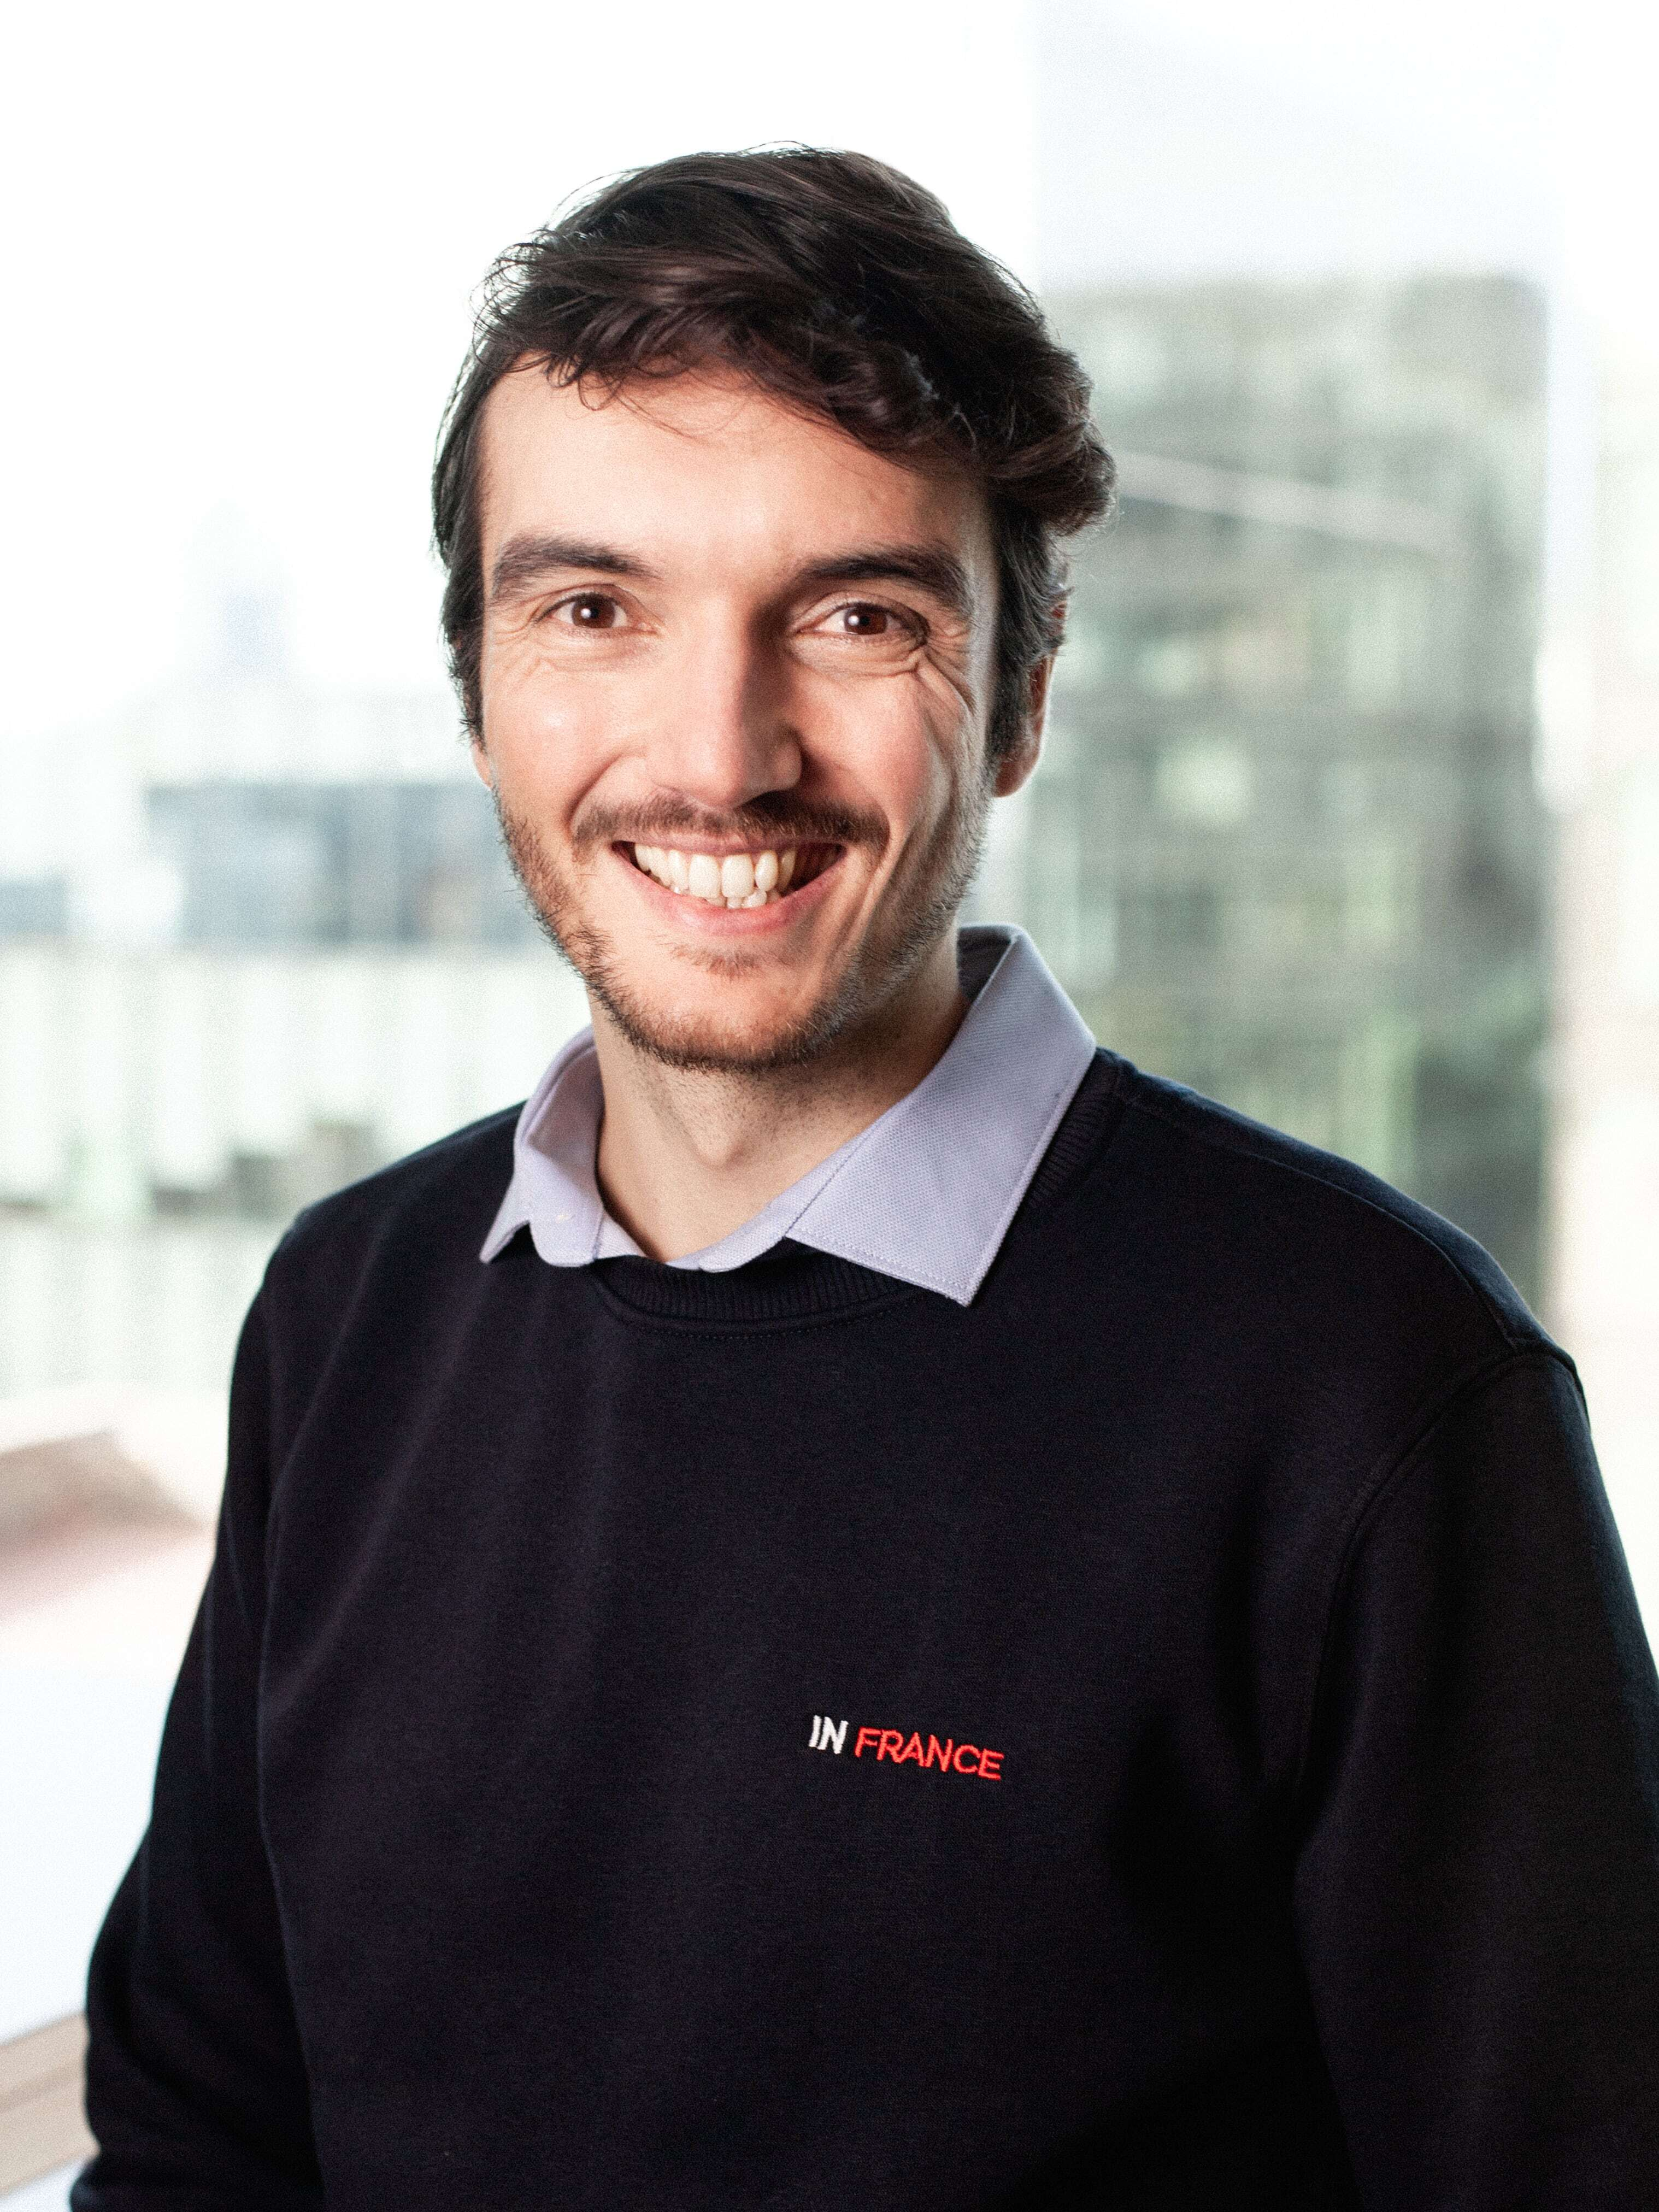
\includegraphics[width=5cm]{image/trombine-christophe}
        \end{columns}
    \end{frame}


    \section{Les ressources du Web}\label{sec:ressources}
    \begin{frame}{Les protocoles}{Websocket, exercice \execcounterdispinc}
        Listez toutes les ressources du Web que vous connaissez.
        \begin{itemize}
            \item ...
        \end{itemize}
        \bigbreak
        \begin{columns}
            \column{0.5\textwidth}
            Restituez-les dans un schéma au formalisme libre (Draw.io est conseillé\ldots).

            \textbf{Prenez le temps de bien nommer chaque concept.}
            \bigbreak
            À présenter au tableau~!
            \column{0.5\textwidth}
            \centering
            
\includegraphics[width=5cm]{image/computer-n-web-ressources}
        \end{columns}
    \end{frame}


    \section{Les protocoles du Web}\label{sec:protocoles}

    \begin{frame}{Les protocoles}{Introductions}
        \footnote{\label{sendbird-protocole}Protocoles de communication WebSocket vs. HTTP, \url{https://sendbird.com/fr/developer/tutorials/websocket-vs-http-communication-protocols}}
        Si on définit le Web comme les applications entre un navigateur et un serveur Web.
        \begin{dangercolorbox}
            Ce qui est très réducteur car il ne prend pas en compte les applications mobiles, les API, les applications desktop, mail, etc.

            Mais c'est l'unique sujet de ce module\ldots
        \end{dangercolorbox}
        Quels sont les protocoles qui permettent à ces applications de communiquer~?
        \pause
        \bigbreak
        Il n'y en a que 2~!
        \begin{itemize}
            \item HTTP(S)
            \item Websocket
        \end{itemize}
    \end{frame}

    \begin{frame}{Les protocoles}{Introduction\label{sendbird-protocole}}
        HTTP, par contre, est un protocole de communication semi-duplex, qui existe depuis un certain temps et constitue la base du Web depuis ses débuts.

        HTTP date de 1989, inventé au CERN par Tim Berners-Lee\footnote{The birth of the Web, \url{https://home.cern/science/computing/birth-web}}. WebSocket est apparu en 2011, inventé par Ian Hickson, également au CERN.
        \bigbreak
        WebSocket, un protocole de communication full-duplex, est relativement plus récent et convient mieux aux applications en temps réel telles (ou presque\ldots) que le live chat dans les applications mobiles, les notifications et oul les appels audio ou vidéo.

        Websocket a été standardisé en 2011\footnote{The WebSocket Protocol, \url{https://datatracker.ietf.org/doc/html/rfc6455}}
    \end{frame}

    \subsection{WebSocket}\label{subsec:websocket}

    \begin{frame}{Les protocoles}{Websocket, exercice \execcounterdispinc}
        \begin{itemize}
            \item Que veut dire full-duplex~?
            \item Y-a-t-il une contradiction avec une architecture client/serveur~?
            \item Citer un autre protocol full-duplex.
            \item Citer un protocol qui \textbf{n'est pas} full-duplex.
        \end{itemize}
        \bigbreak
        \centering
        
\includegraphics[width=5cm]{image/homework}
    \end{frame}

    \begin{frame}{Les protocoles}{Websocket\label{sendbird-protocole}}
        \centering
        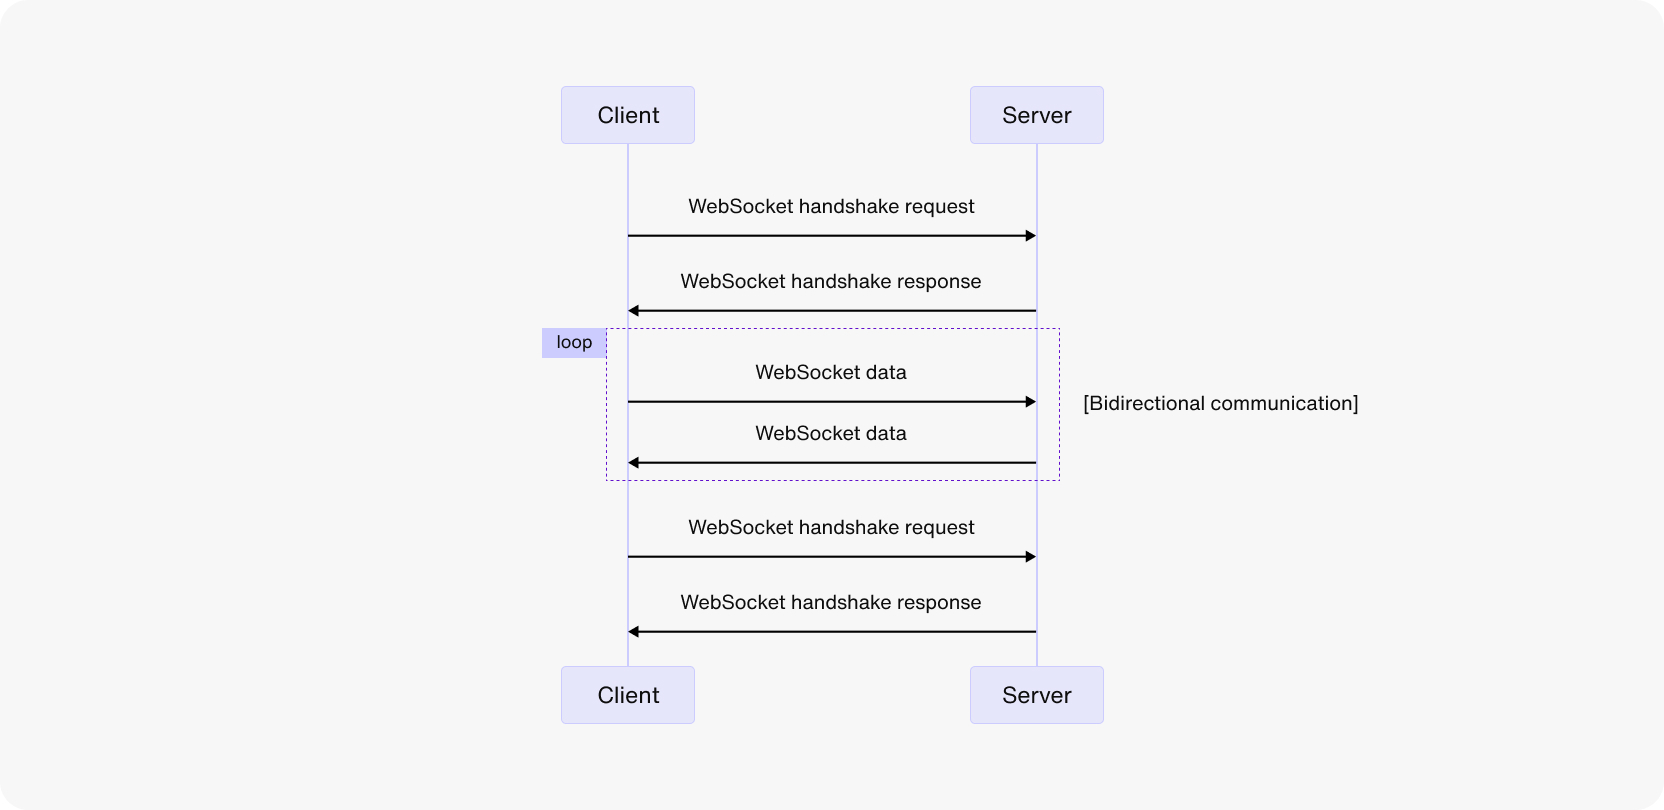
\includegraphics[width=12cm]{image/tutorial-websocket-protocol-chart}
    \end{frame}

    \begin{frame}{Les protocoles}{Websocket côté client (Navigateur)\footnote{\label{mozilla-websocket}WebSockets, \url{https://developer.mozilla.org/fr/docs/Web/API/WebSockets_API}}}
        \begin{columns}
            \column{0.5\textwidth}
            \centering
            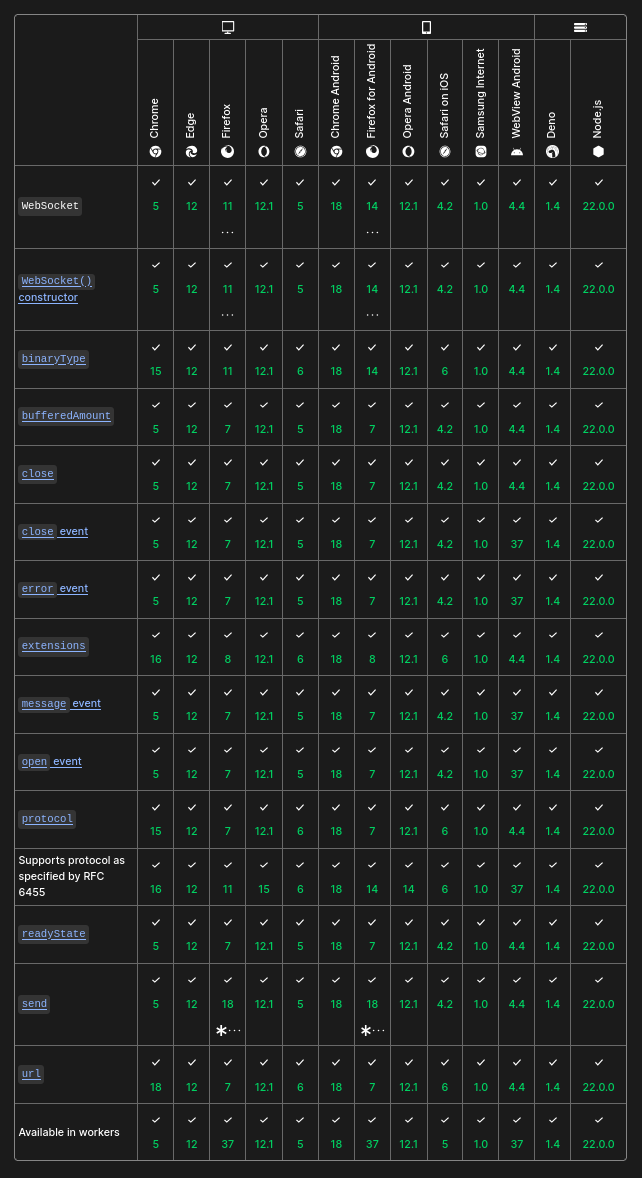
\includegraphics[width=3.3cm]{image/client-support} \\ Client \\
            \column{0.5\textwidth}
            \centering
            
\includegraphics[width=6.5cm]{image/kids-on-the-phone}
        \end{columns}
    \end{frame}

    \begin{frame}{Les protocoles}{Websocket côté serveur (liste non exhaustive !)\cref{mozilla-websocket}}
        \begin{scriptsize}
            \begin{itemize}

                \item \href{https://github.com/uWebSockets/uWebSockets}{µWebSockets}~: Déclinaison plus légère et plus performante de WebSocket et écrite en \href{https://isocpp.org/}{C++11} et en \href{https://nodejs.org/fr/}{Node.js}.

                \item \href{https://github.com/ClusterWS/ClusterWS}{ClusteWS~}: Framework léger, rapide et puissant qui permet de construire des application en \href{https://nodejs.org/fr/}{Node.js}.

                \item \href{http://socket.io}{Socket.IO}~: API WebSocket puissante et multiplateformes en \href{https://nodejs.org}{Node.js}.

                \item \href{https://socketcluster.io/\#!/}{SocketCluster}~: Framework open source en temps réel en \href{https://nodejs.org}{Node.js}.

                \item \href{https://nodejs.org}{Node.js}.

                \item \href{https://www.totaljs.com/}{Total.js}~: FrameWork pour web application en \href{https://nodejs.org}{Node.js}.

                \item \href{https://www.npmjs.com/package/faye-websocket}{Faye}~: Combine WebSocket(bidirectionnelle) et EventSource(unidirectionnelle), côté serveur et côté client en \href{https://nodejs.org}{Node.js}.

                \item \href{https://signalr.net/}{SignalR}~: SignalR est une nouvelle bibliothèque pour les développeurs \href{https://dotnet.microsoft.com/apps/aspnet}{ASP.NET}.

                \item \href{https://caddyserver.com/docs/websocket}{Caddy}~: Serveur web capable de créer des WebSockets serveur/proxy(stdin/stdout, echo, cat, \ldots).

                \item \href{https://github.com/websockets/ws}{ws}~: La plus populaire des WebSockets pour client \& serveur en \href{https://nodejs.org}{Node.js}.

                \item \href{https://github.com/bigstepinc/jsonrpc-bidirectional}{jsonrpc-bidirectional}~: Implémentation de JSON-RPC 2.0 sur WebSocket.

                \item \href{https://github.com/ninenines/cowboy}{cowboy}~: Cowboy est un petit serveur HTTP rapide et moderne pour Erlang/OTP basé sur WebSocket.

                \item \href{https://zeromq.org}{ZeroMQ}~: ZeroMQ est une bibliothèque de fonctions pour transporter des messages avec divers protocoles IPC, TCP, UDP, TIPC, diffusion de groupe et WebSocket.

            \end{itemize}
        \end{scriptsize}
    \end{frame}

    \begin{frame}{Les protocoles}{Websocket, exercice \execcounterdispinc}
        Dans un groupe de deux ou trois~:
        \begin{itemize}
            \item Développer une page HTML avec un Javascript se connectant à un serveur WebSocket avec la techno/librairie de votre choix.
            \item Développer un serveur WebSocket avec la techno/librairie de votre choix.
            \item Les livrables, codes source commentés et captures d'écran, sont à déposer dans Teams.
        \end{itemize}
        \begin{dangercolorbox}
            À la vue de l'omniprésence de ce protocole sur de nombreuses technos et de la bonne compatibilité des méthodes.
            Est-il nécessaire d'utiliser des librairies (dépendances logicielles)~?
        \end{dangercolorbox}
    \end{frame}

    \subsection{HTTP}\label{subsec:http}

    \begin{frame}{Les protocoles}{HTTP\label{sendbird-protocole}}
        \centering
        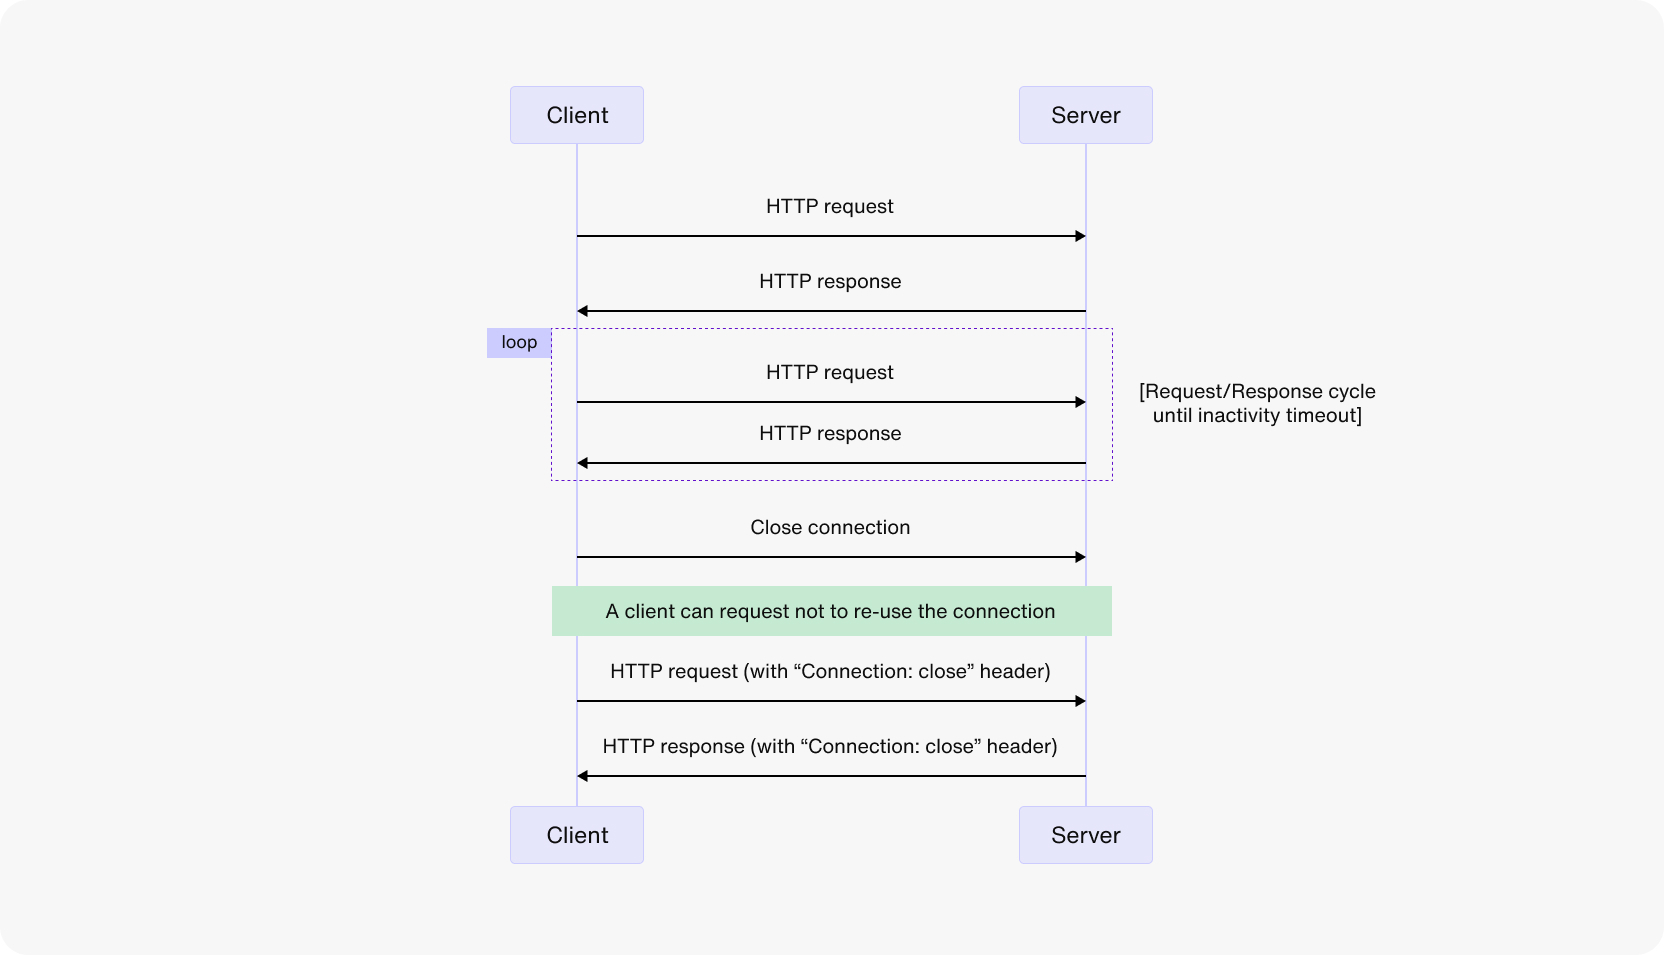
\includegraphics[width=12cm]{image/Tutorial-HTTP-connection-chart}
    \end{frame}

    \subsection{WebSocket VS HTTP}\label{subsec:ws-vs-http}

    \begin{frame}{Les protocoles}{HTTP\label{sendbird-protocole}}
        \centering
        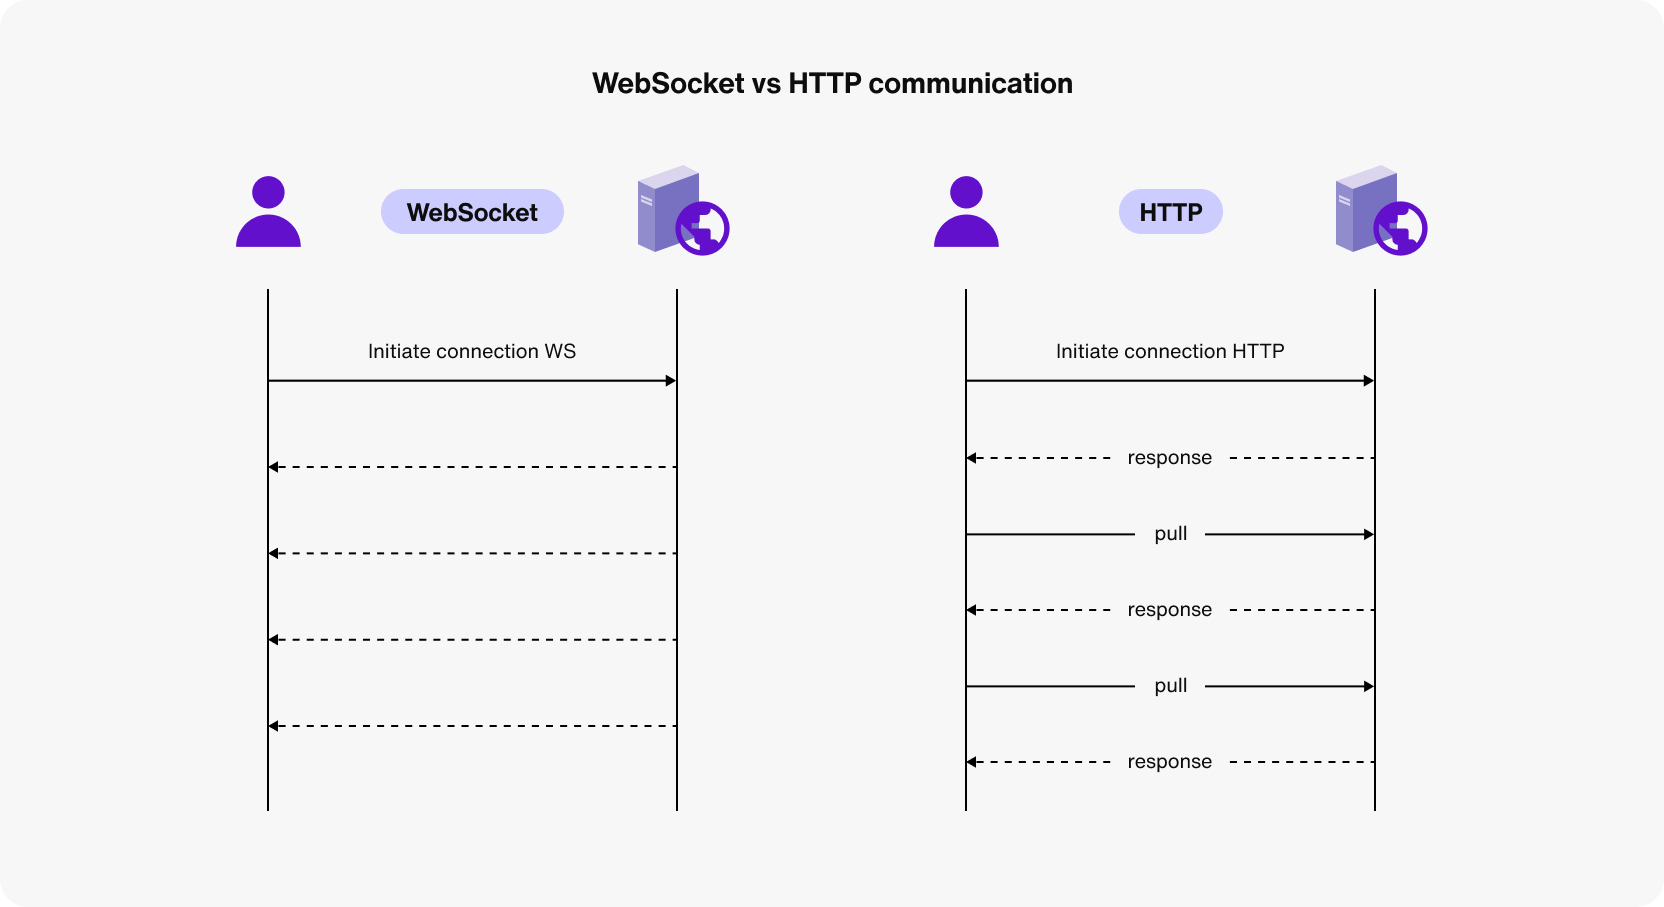
\includegraphics[width=12cm]{image/Tutorial-WebSocket-vs.-HTTP-communication-diagram}
    \end{frame}


    \section{Licence CC}\label{sec:licence}

    \begin{frame}{Licence}{Licence Creative Commons}
        Support de cours sous licence Creative Commons BY-NC-ND~.
        \bigbreak
        Vous pouvez donc, partager, copier, distribuer le document.
        \bigbreak
        Attribution requise à PapIT SASU - Pas d’utilisation commerciale - Pas de modification
        \bigbreak
        \centering
        
\includegraphics[width=5cm]{image/by-nc-nd-logo}
    \end{frame}
\end{document}
